\documentclass[11pt, a4paper]{article}
\usepackage{pdfpages}
\usepackage{parallel}
\usepackage[T2A]{fontenc}
\usepackage{ucs}
\usepackage[utf8x]{inputenc}
\usepackage[polish,english,russian]{babel}
\usepackage{hyperref}
\usepackage{rotating}
\usepackage[inner=2cm,top=1.8cm,outer=2cm,bottom=2.3cm,nohead]{geometry}
\usepackage{listings}
\usepackage{graphicx}
\usepackage{wrapfig}
\usepackage{longtable}
\usepackage{indentfirst}
\usepackage{array}
\usepackage{tikzsymbols}
\usepackage{soul}
\usepackage[ruled,vlined]{algorithm2e}
%\counterwithout{figure}{section} 

\usepackage{url}
\makeatletter
\g@addto@macro{\UrlBreaks}{\UrlOrds}
\makeatother

\newcolumntype{P}[1]{>{\raggedright\arraybackslash}p{#1}}
\frenchspacing
\usepackage{fixltx2e} %text sub- and superscripts
\usepackage{icomma} % коскі ў матэматычным рэжыме
\PreloadUnicodePage{4}

\newcommand{\longpage}{\enlargethispage{\baselineskip}}
\newcommand{\shortpage}{\enlargethispage{-\baselineskip}}

\def\switchlang#1{\expandafter\csname switchlang#1\endcsname}
\def\switchlangbe{
\let\saverefname=\refname%
\def\refname{Літаратура}%
\def\figurename{Іл.}%
}
\def\switchlangen{
\let\saverefname=\refname%
\def\refname{References}%
\def\figurename{Fig.}%
}
\def\switchlangru{
\let\saverefname=\refname%
\let\savefigurename=\figurename%
\def\refname{Литература}%
\def\figurename{Рис.}%
}

\hyphenation{admi-ni-stra-tive}
\hyphenation{ex-pe-ri-ence}
\hyphenation{fle-xi-bi-li-ty}
\hyphenation{Py-thon}
\hyphenation{ma-the-ma-ti-cal}
\hyphenation{re-ported}
\hyphenation{imp-le-menta-tions}
\hyphenation{pro-vides}
\hyphenation{en-gi-neering}
\hyphenation{com-pa-ti-bi-li-ty}
\hyphenation{im-pos-sible}
\hyphenation{desk-top}
\hyphenation{elec-tro-nic}
\hyphenation{com-pa-ny}
\hyphenation{de-ve-lop-ment}
\hyphenation{de-ve-loping}
\hyphenation{de-ve-lop}
\hyphenation{da-ta-ba-se}
\hyphenation{plat-forms}
\hyphenation{or-ga-ni-za-tion}
\hyphenation{pro-gramming}
\hyphenation{in-stru-ments}
\hyphenation{Li-nux}
\hyphenation{sour-ce}
\hyphenation{en-vi-ron-ment}
\hyphenation{Te-le-pathy}
\hyphenation{Li-nux-ov-ka}
\hyphenation{Open-BSD}
\hyphenation{Free-BSD}
\hyphenation{men-ti-on-ed}
\hyphenation{app-li-ca-tion}

\def\progref!#1!{\texttt{#1}}
\renewcommand{\arraystretch}{2} %Іначай формулы ў матрыцы зліпаюцца з лініямі
\usepackage{array}

\def\interview #1 (#2), #3, #4, #5\par{

\section[#1, #3, #4]{#1 -- #3, #4}
\def\qname{LVEE}
\def\aname{#1}
\def\q ##1\par{{\noindent \bf \qname: ##1 }\par}
\def\a{{\noindent \bf \aname: } \def\qname{L}\def\aname{#2}}
}

\def\interview* #1 (#2), #3, #4, #5\par{

\section*{#1\\{\small\rm #3, #4. #5}}
\ifx\ParallelWhichBox\undefined%
    \addcontentsline{toc}{section}{#1, #3, #4}%
\else%
\ifnum\ParallelWhichBox=0%
    \addcontentsline{toc}{section}{#1, #3, #4}%
\fi\fi%

\def\qname{LVEE}
\def\aname{#1}
\def\q ##1\par{{\noindent \bf \qname: ##1 }\par}
\def\a{{\noindent \bf \aname: } \def\qname{L}\def\aname{#2}}
}

\newcommand{\interviewfooter}[1]{
\vskip 1em
\noindent \textit{#1}
}

\switchlang{en}
\begin{document}

\title{1983 "--- Hawley Mark II X063X Mouse}
\date{}
\maketitle
\selectlanguage{english}
The Mark II X063X Mouse (figure \ref{fig:HawleyMarkIIPic}) was the first in-house development of the Hawley Mouse House \cite{hawley,mouses} by Jack Hawley, co-designer of the Xerox Alto computer mouse and co-author of the 1973 Xerox patent for mouse with two inclined wheels \cite{pat}.

\begin{figure}[h]
   \centering
    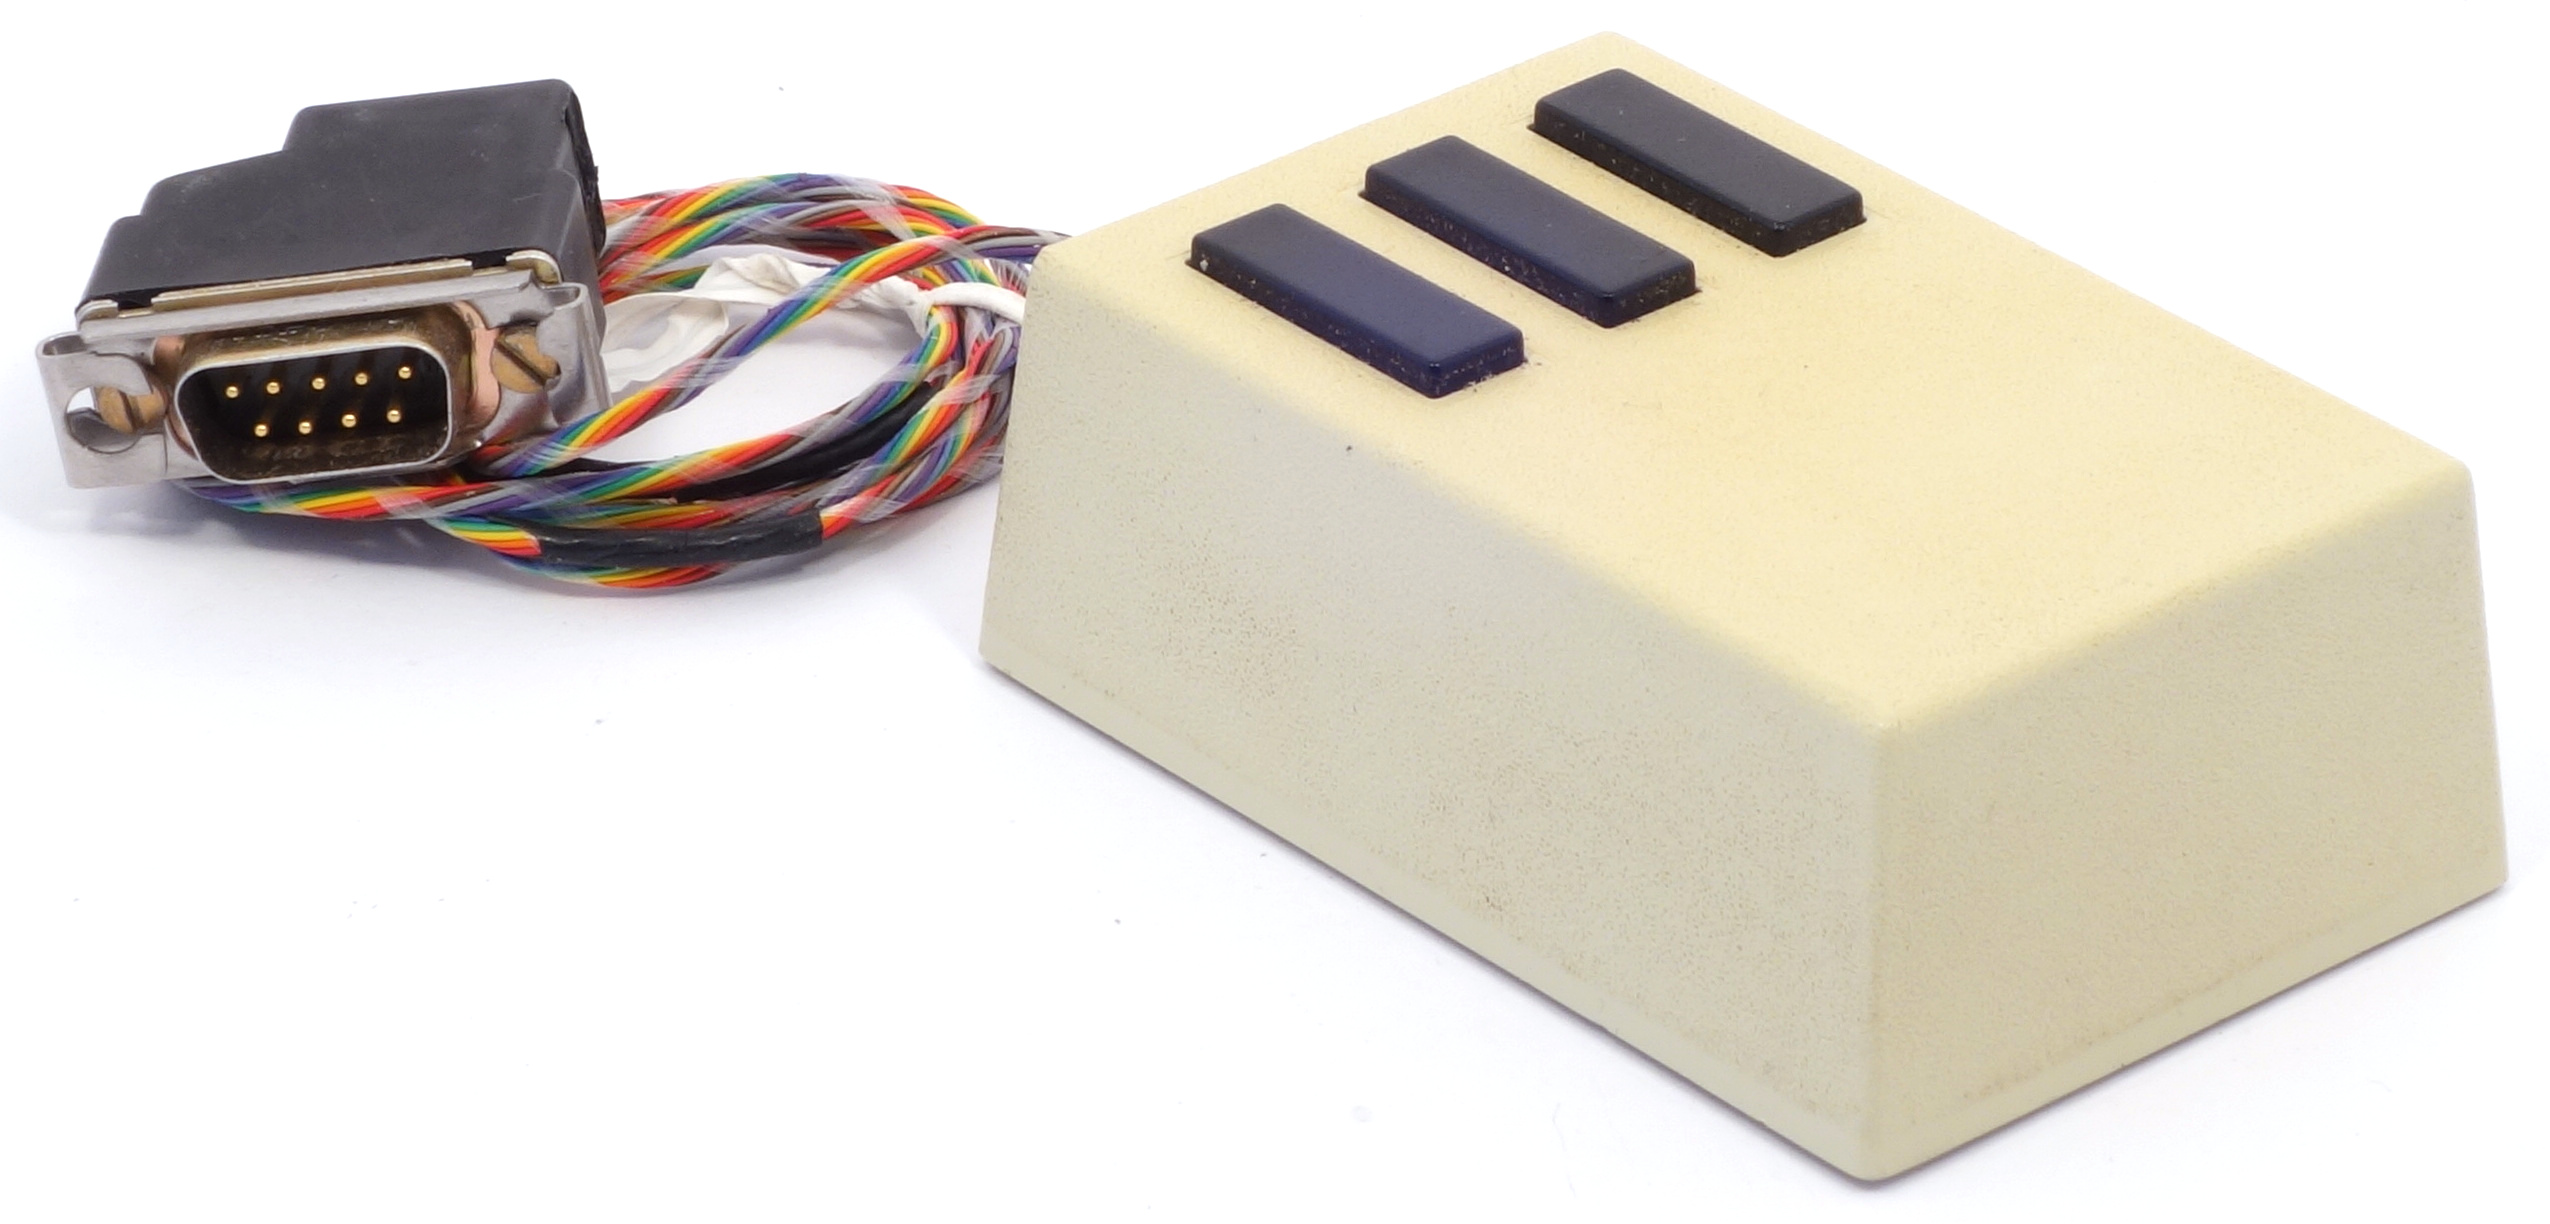
\includegraphics[scale=0.6]{1983_hawley_mark_ii/pic_60.jpg}
    \caption{Hawley Mark II X063X Mouse}
    \label{fig:HawleyMarkIIPic}
\end{figure}

The Mark II X063X mouse is made in an industrial design brought to an extreme degree: the body is an almost regular parallelepiped, on which there are three rectangular buttons with the most contrasting color in relation to the body (figure \ref{fig:HawleyMarkIITopAndBottom}). Obviously, the design was intended to emphasize the purpose of the mouse, aimed at engineers and users of various CAD systems (including solid modeling and architecture).

This item is beige with black buttons (on the cable you can see the remnants of black insulation, which has lost its elasticity over time and crumbled to pieces). The variant with the opposite combination of body and button colors was also common, and several more color options are known. The Hawley advertising gives an idea of the color combinations \cite{brochure}, but there is no information on how many color combinations from this promotional ad were actually implemented.

\begin{figure}[h]
    \centering
    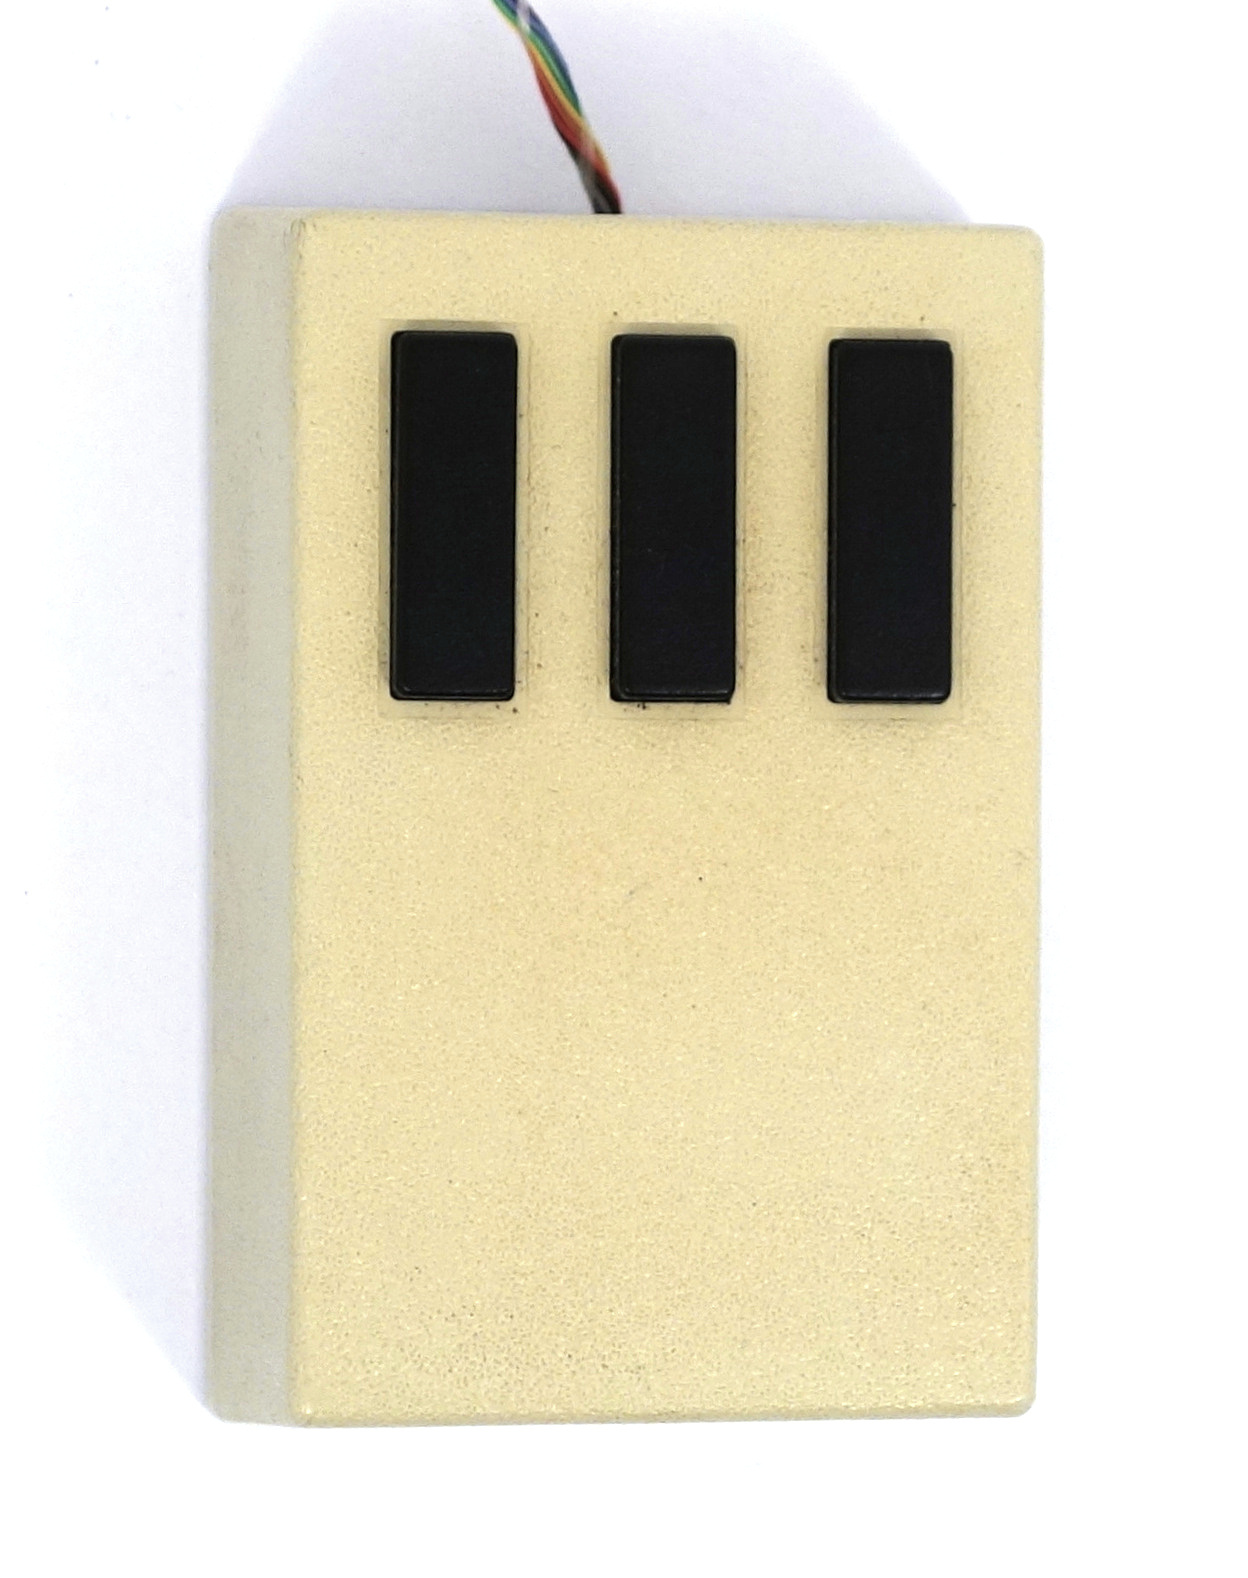
\includegraphics[scale=0.5]{1983_hawley_mark_ii/top_60.jpg}
    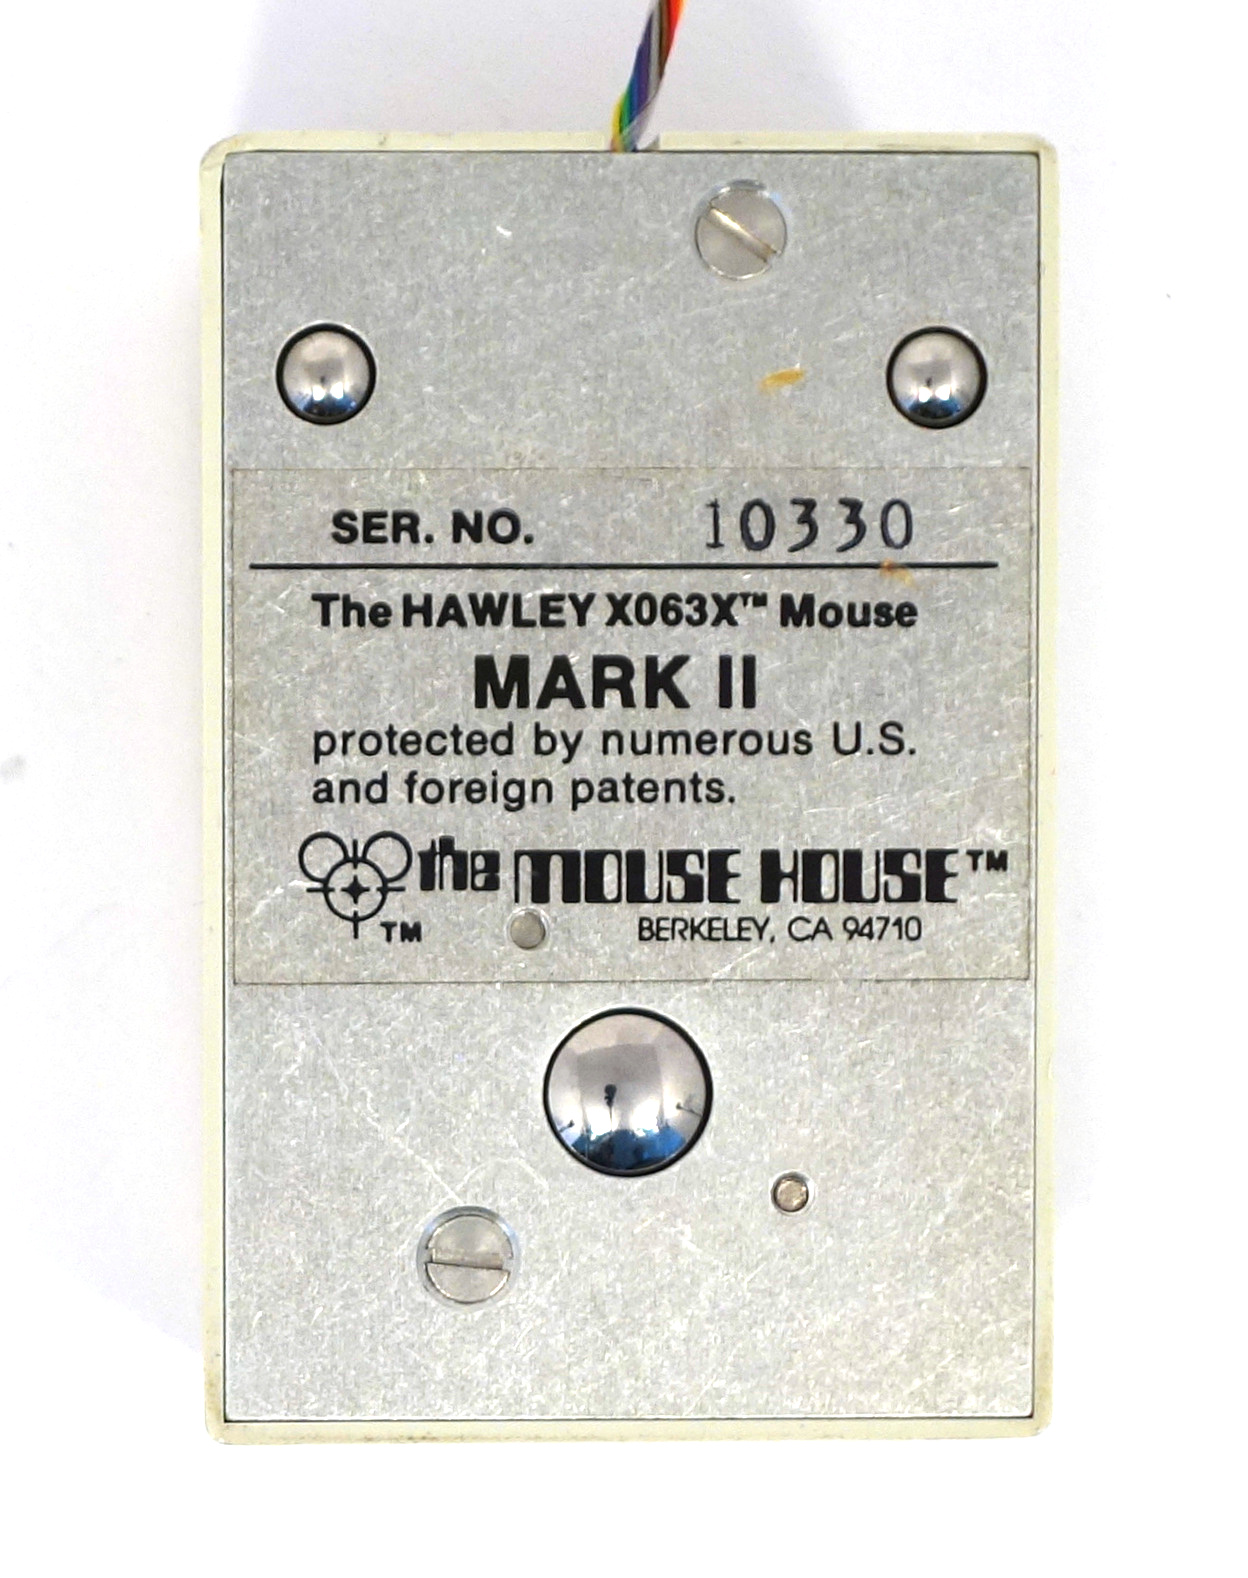
\includegraphics[scale=0.5]{1983_hawley_mark_ii/bottom_60.jpg}
    \caption{Hawley Mark II X063X Mouse, top and bottom views}
    \label{fig:HawleyMarkIITopAndBottom}
\end{figure}



Bottom side is entirely made of metal (figure \ref{fig:HawleyMarkIITopAndBottom}). Rotation is registered by a smooth steel ball in the center, while two smaller balls act as feet to minimize friction. A removable ring that allows you to remove the ball to remove collected debris is not yet provided in this model, so complete disassembly is necessary for cleaning.

\begin{figure}[h]
    \centering
    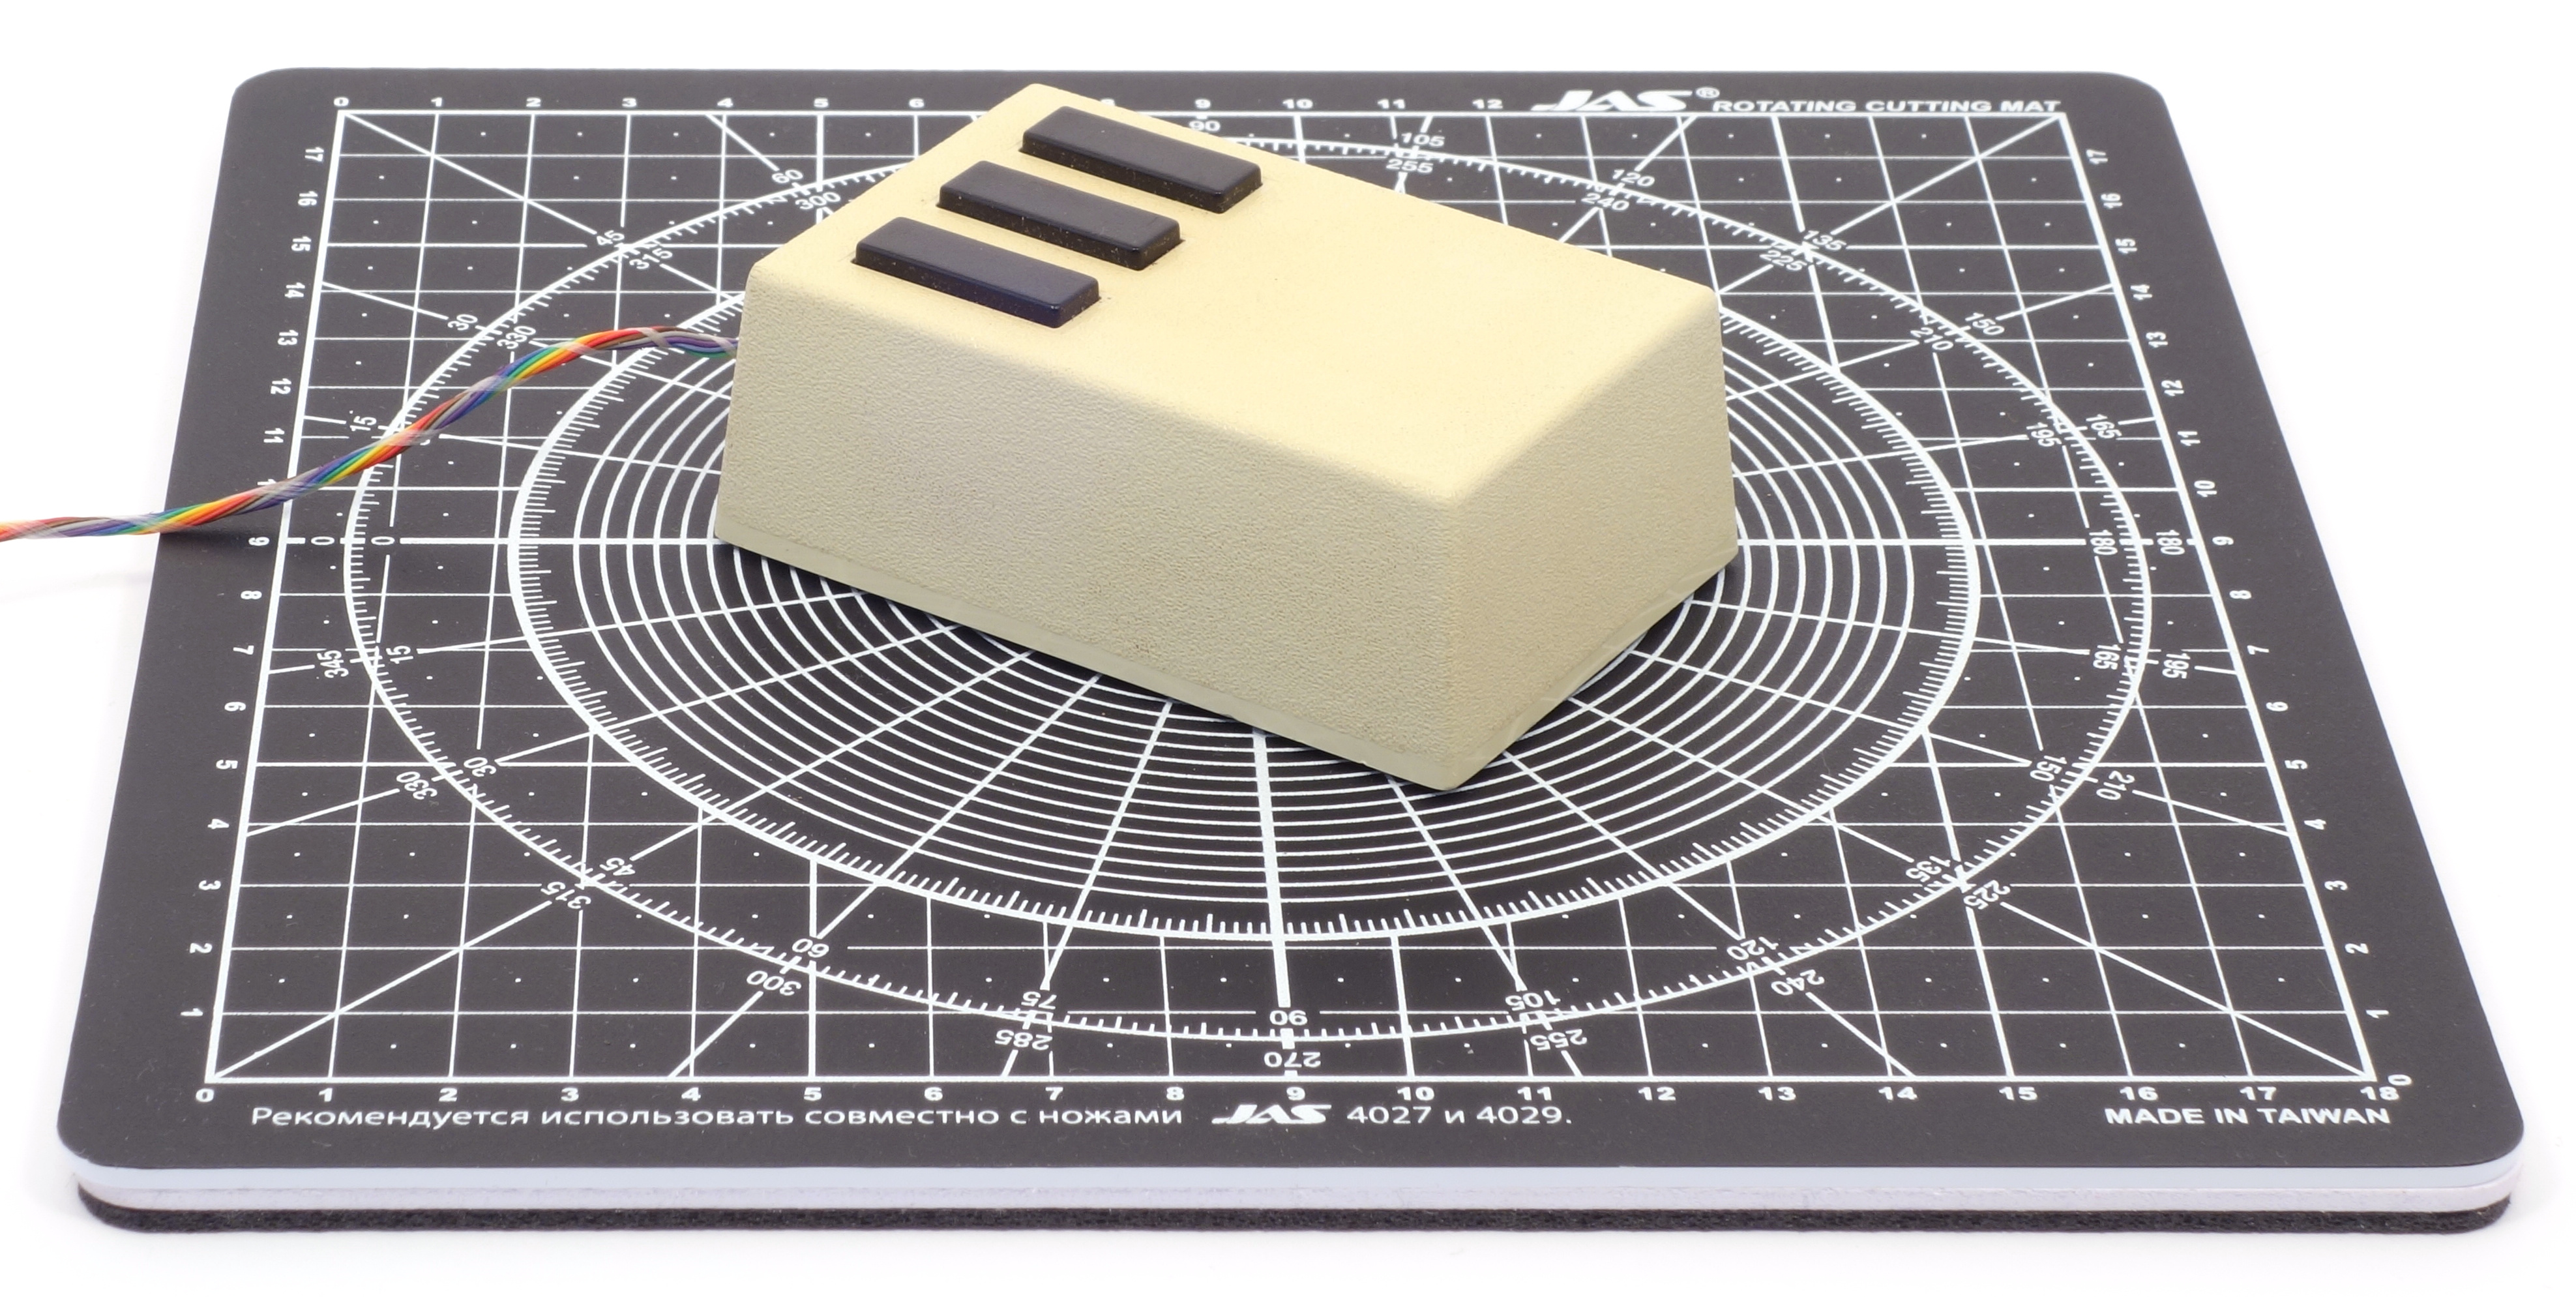
\includegraphics[scale=0.5]{1983_hawley_mark_ii/size_30.jpg}
    \caption{Hawley Mark II on a graduated pad with a grid step of 1~cm}
    \label{fig:HawleyMarkIISize}
\end{figure}

The mouse has a small size, typical for mice of the 1980s (figure \ref{fig:HawleyMarkIISize}). Obviously, this at least slightly reduces the negative impact of the body with orthogonal edges on ergonomics, since the hand can only lean on the body to a small extent (figure \ref{fig:HawleyMarkIIHand}).

\begin{figure}[h]
    \centering
    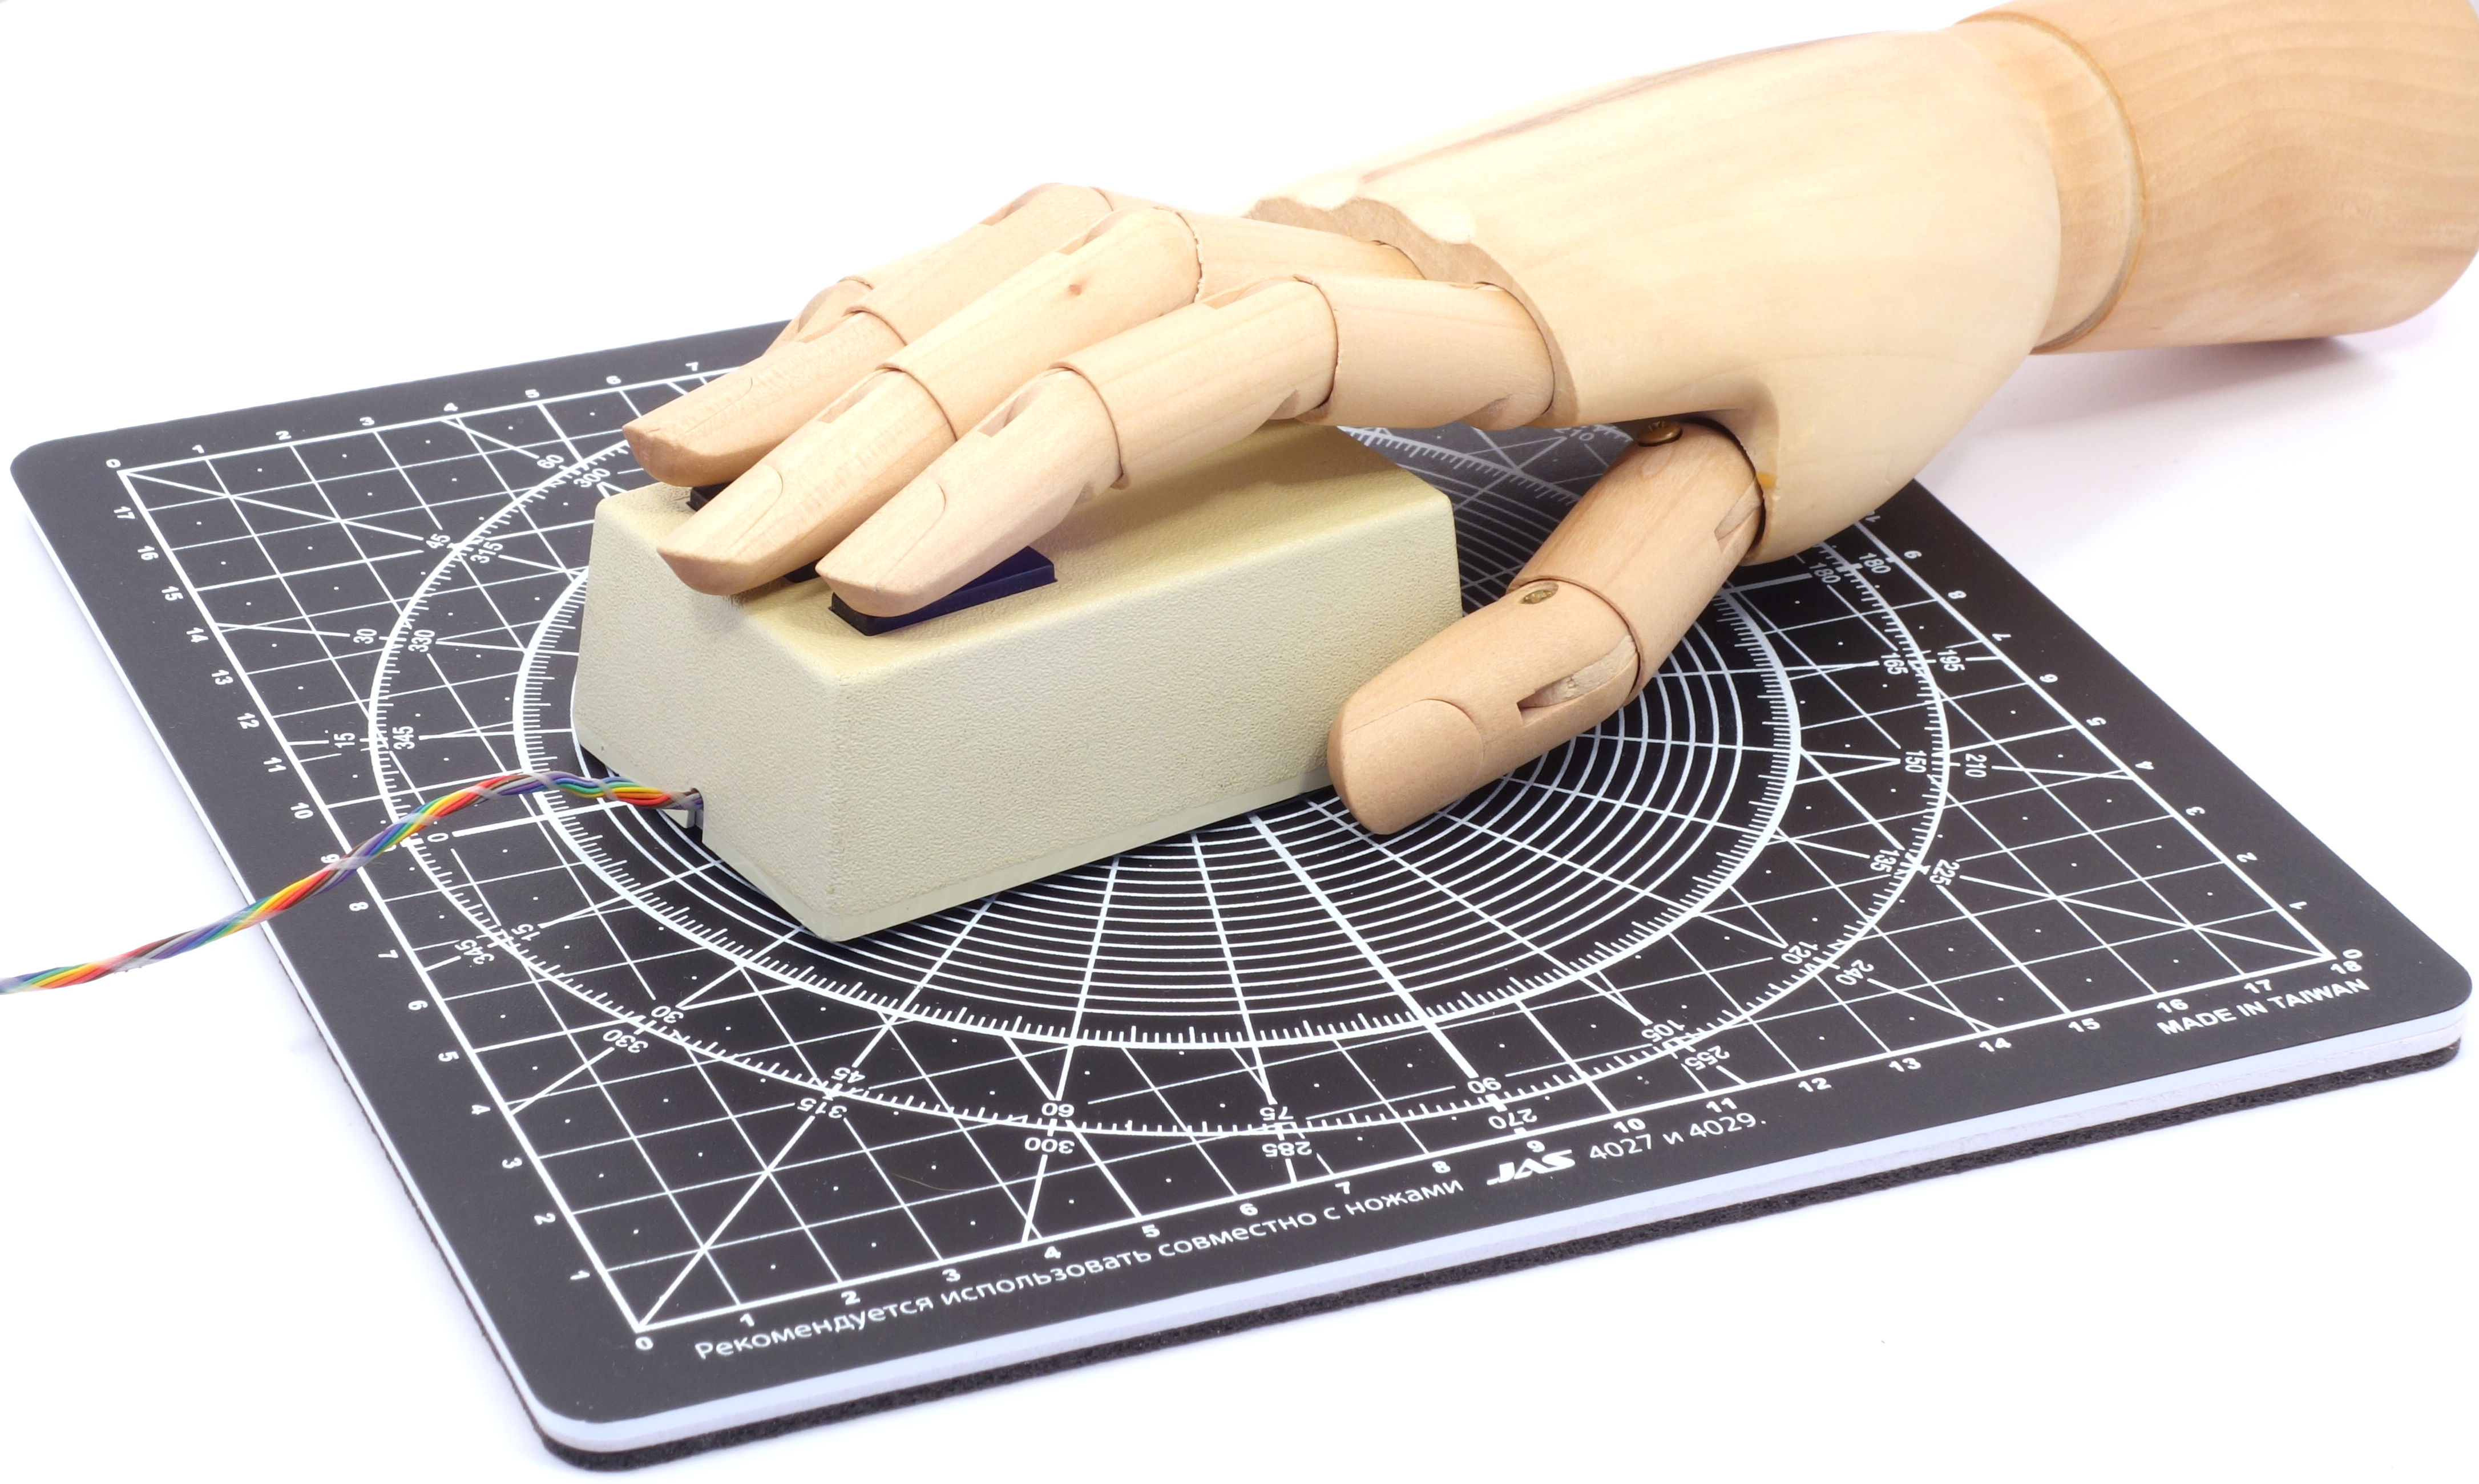
\includegraphics[scale=0.5]{1983_hawley_mark_ii/hand_60.jpg}
    \caption{Hawley Mark II with a human hand model}
    \label{fig:HawleyMarkIIHand}
\end{figure}

Mouse internals are shown in figure \ref{fig:HawleyMarkIIInside}. The removable solid protection of the ball is worthy of mention: it requires additional disassembly operations to remove garbage. In this mouse, contact encoders (with four contacts for greater reliability) are used, which are based on a metal contact drum instead of the more common disk in subsequent models.

 \begin{figure}[h]
    \centering
    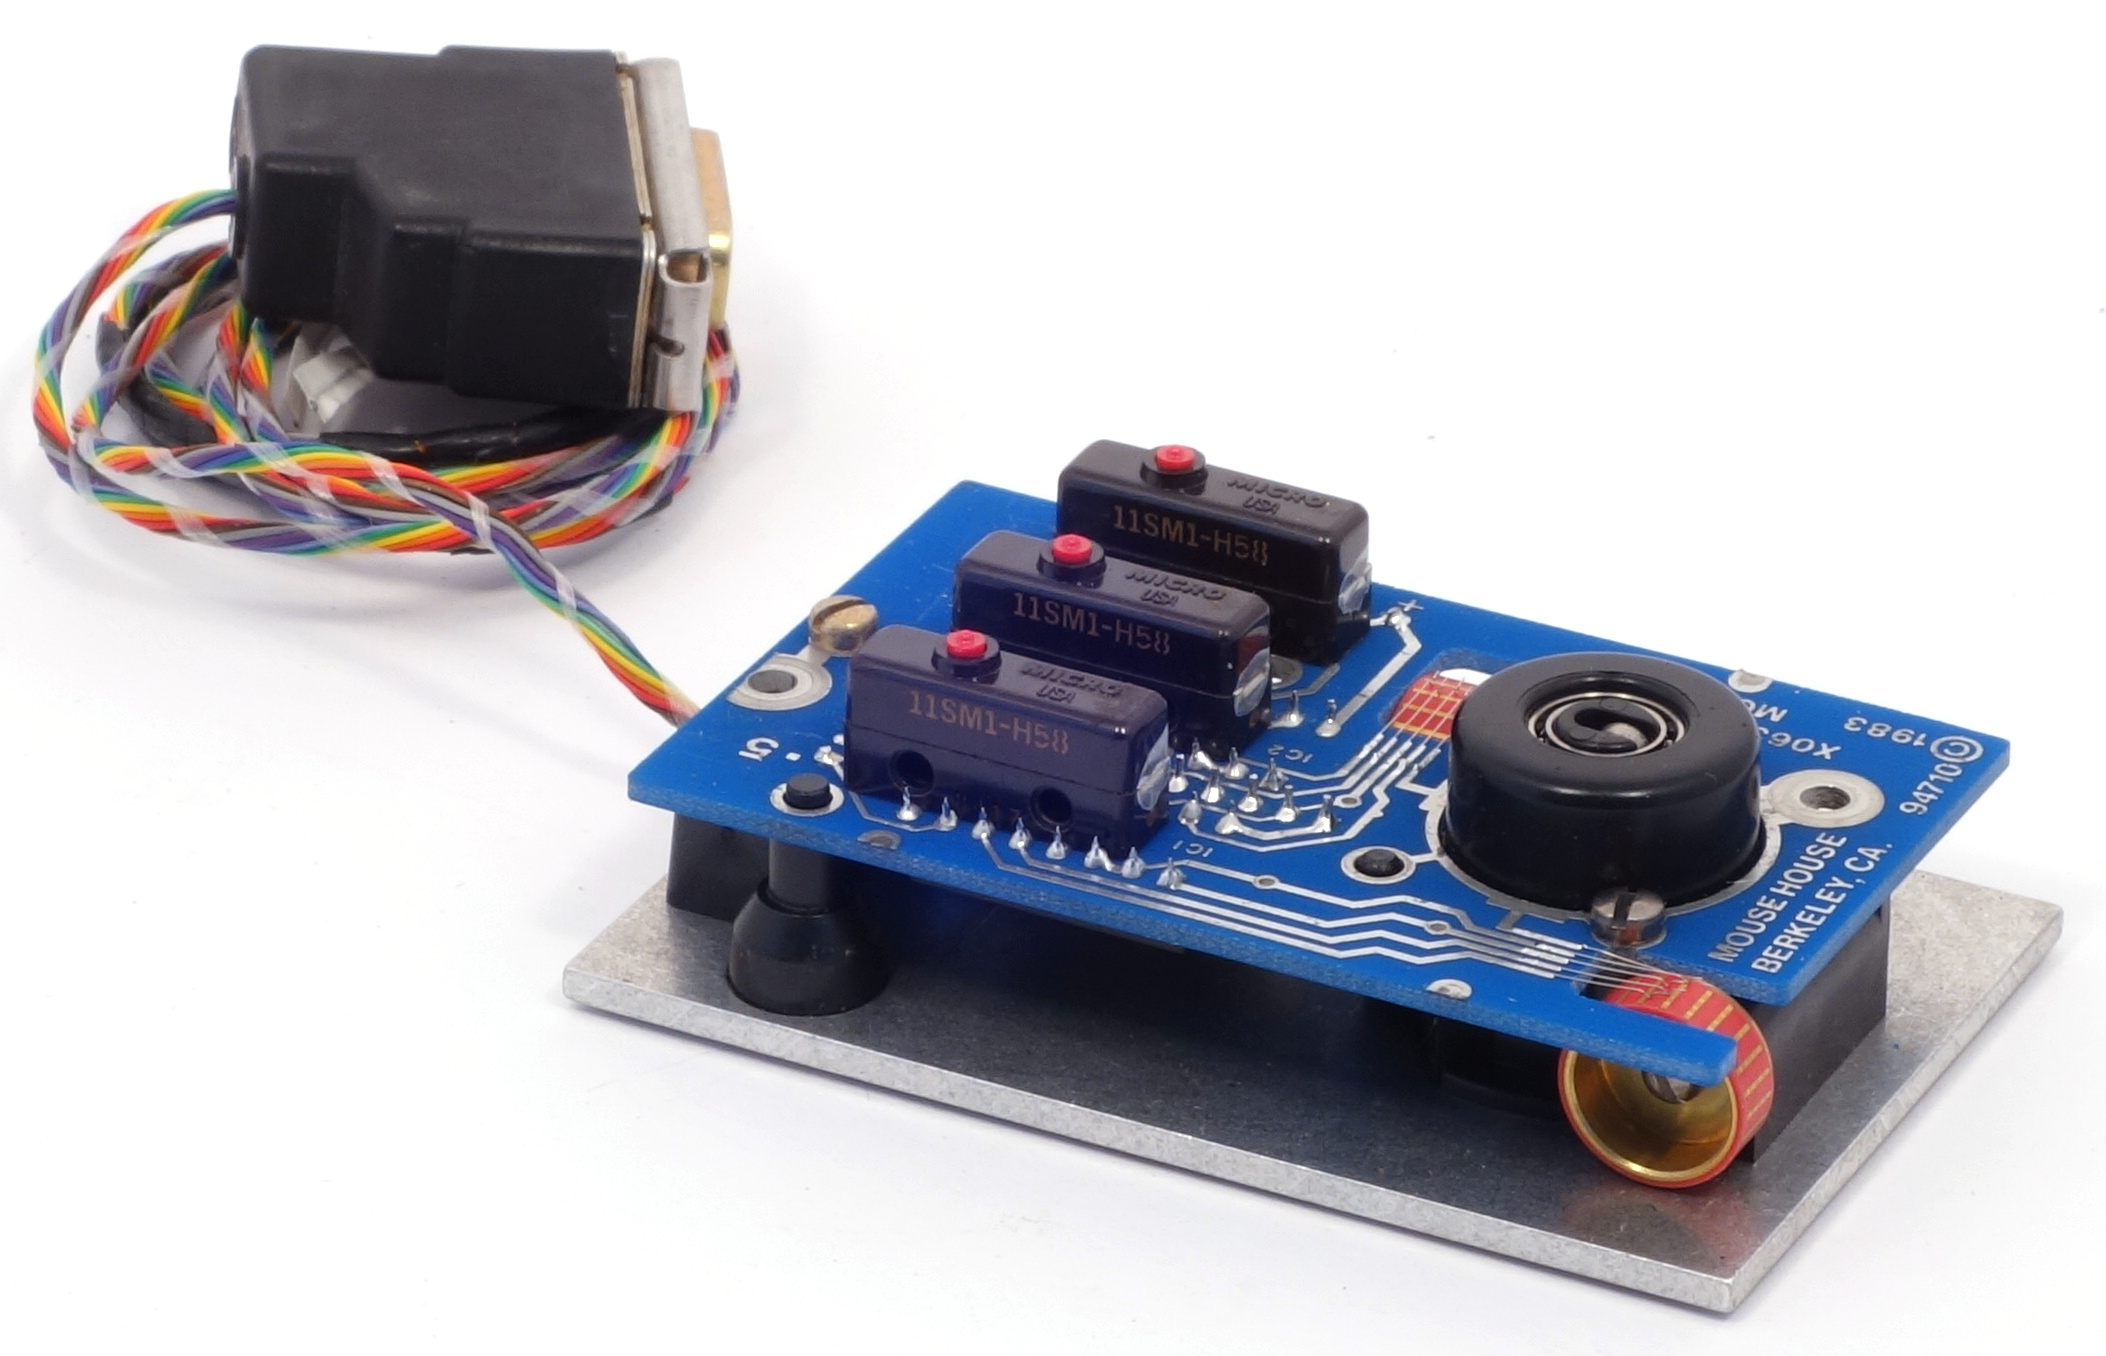
\includegraphics[scale=0.8]{1983_hawley_mark_ii/inside_60.jpg}
    \caption{Hawley Mark II disassembled}
    \label{fig:HawleyMarkIIInside}
\end{figure}

\begin{thebibliography}{9}
\bibitem{hawley} Hawley Mouse House \url{https://oldmouse.com/mouse/hawley/}

\bibitem{mouses} Hawley Mark II X063X Mouses \url{https://oldmouse.com/mouse/hawley/X063X.shtml}

\bibitem{pat} Transducer for a display-oriented pointing device \url{https://patents.google.com/patent/US3892963A/en}

\bibitem{brochure} Mouse House MK II Brochure \url{https://www.microsoft.com/buxtoncollection/a/pdf/Mouse%20House%20MK%20II%20Brochure.pdf}
\end{thebibliography}
\end{document}
